% Options for packages loaded elsewhere
\PassOptionsToPackage{unicode}{hyperref}
\PassOptionsToPackage{hyphens}{url}
%
\documentclass[
  9pt,
]{extbook}
\usepackage{lmodern}
\usepackage{amsmath}
\usepackage{ifxetex,ifluatex}
\ifnum 0\ifxetex 1\fi\ifluatex 1\fi=0 % if pdftex
  \usepackage[T1]{fontenc}
  \usepackage[utf8]{inputenc}
  \usepackage{textcomp} % provide euro and other symbols
  \usepackage{amssymb}
\else % if luatex or xetex
  \usepackage{unicode-math}
  \defaultfontfeatures{Scale=MatchLowercase}
  \defaultfontfeatures[\rmfamily]{Ligatures=TeX,Scale=1}
\fi
% Use upquote if available, for straight quotes in verbatim environments
\IfFileExists{upquote.sty}{\usepackage{upquote}}{}
\IfFileExists{microtype.sty}{% use microtype if available
  \usepackage[]{microtype}
  \UseMicrotypeSet[protrusion]{basicmath} % disable protrusion for tt fonts
}{}
\makeatletter
\@ifundefined{KOMAClassName}{% if non-KOMA class
  \IfFileExists{parskip.sty}{%
    \usepackage{parskip}
  }{% else
    \setlength{\parindent}{0pt}
    \setlength{\parskip}{6pt plus 2pt minus 1pt}}
}{% if KOMA class
  \KOMAoptions{parskip=half}}
\makeatother
\usepackage{xcolor}
\IfFileExists{xurl.sty}{\usepackage{xurl}}{} % add URL line breaks if available
\IfFileExists{bookmark.sty}{\usepackage{bookmark}}{\usepackage{hyperref}}
\hypersetup{
  pdftitle={The Live Textbook of Physical Chemistry 2},
  pdfauthor={Dr.~Roberto Peverati},
  hidelinks,
  pdfcreator={LaTeX via pandoc}}
\urlstyle{same} % disable monospaced font for URLs
\usepackage{longtable,booktabs}
\usepackage{calc} % for calculating minipage widths
% Correct order of tables after \paragraph or \subparagraph
\usepackage{etoolbox}
\makeatletter
\patchcmd\longtable{\par}{\if@noskipsec\mbox{}\fi\par}{}{}
\makeatother
% Allow footnotes in longtable head/foot
\IfFileExists{footnotehyper.sty}{\usepackage{footnotehyper}}{\usepackage{footnote}}
\makesavenoteenv{longtable}
\usepackage{graphicx}
\makeatletter
\def\maxwidth{\ifdim\Gin@nat@width>\linewidth\linewidth\else\Gin@nat@width\fi}
\def\maxheight{\ifdim\Gin@nat@height>\textheight\textheight\else\Gin@nat@height\fi}
\makeatother
% Scale images if necessary, so that they will not overflow the page
% margins by default, and it is still possible to overwrite the defaults
% using explicit options in \includegraphics[width, height, ...]{}
\setkeys{Gin}{width=\maxwidth,height=\maxheight,keepaspectratio}
% Set default figure placement to htbp
\makeatletter
\def\fps@figure{htbp}
\makeatother
\setlength{\emergencystretch}{3em} % prevent overfull lines
\providecommand{\tightlist}{%
  \setlength{\itemsep}{0pt}\setlength{\parskip}{0pt}}
\setcounter{secnumdepth}{5}
\usepackage{booktabs}
\usepackage{pdfpages}
\usepackage{amsthm}
\usepackage[version=4]{mhchem}
\usepackage{cancel}

%change to a smaller page:
\usepackage[paperwidth=6in, paperheight=9in]{geometry}
% this is to change the size of text: headsep=10pt, textheight=550pt
%\usepackage[textwidth=456pt]{geometry}

%fancyhdr to set custom headers for the book:
\usepackage{fancyhdr}
\pagestyle{fancy}
\fancyhf{}
\fancyhead[LO]{\slshape\nouppercase{\rightmark}}
\fancyhead[RE]{\slshape\nouppercase{\leftmark}}
\fancyhead[RO,LE]{\thepage}

\makeatletter
\def\thm@space@setup{%
  \thm@preskip=8pt plus 2pt minus 4pt
  \thm@postskip=\thm@preskip
}
\makeatother
\let\oldmaketitle\maketitle
\AtBeginDocument{\let\maketitle\relax}
\ifluatex
  \usepackage{selnolig}  % disable illegal ligatures
\fi
\usepackage[]{natbib}
\bibliographystyle{apalike}

\title{The Live Textbook of Physical Chemistry 2}
\author{\href{mailto:rpeverati@fit.edu}{Dr.~Roberto Peverati}}
\date{10 January 2021}

\usepackage{amsthm}
\newtheorem{theorem}{Theorem}[chapter]
\newtheorem{lemma}{Lemma}[chapter]
\newtheorem{corollary}{Corollary}[chapter]
\newtheorem{proposition}{Proposition}[chapter]
\newtheorem{conjecture}{Conjecture}[chapter]
\theoremstyle{definition}
\newtheorem{definition}{Definition}[chapter]
\theoremstyle{definition}
\newtheorem{example}{Example}[chapter]
\theoremstyle{definition}
\newtheorem{exercise}{Exercise}[chapter]
\theoremstyle{remark}
\newtheorem*{remark}{Remark}
\newtheorem*{solution}{Solution}
\begin{document}
\maketitle

%Frontpage for 6x9:
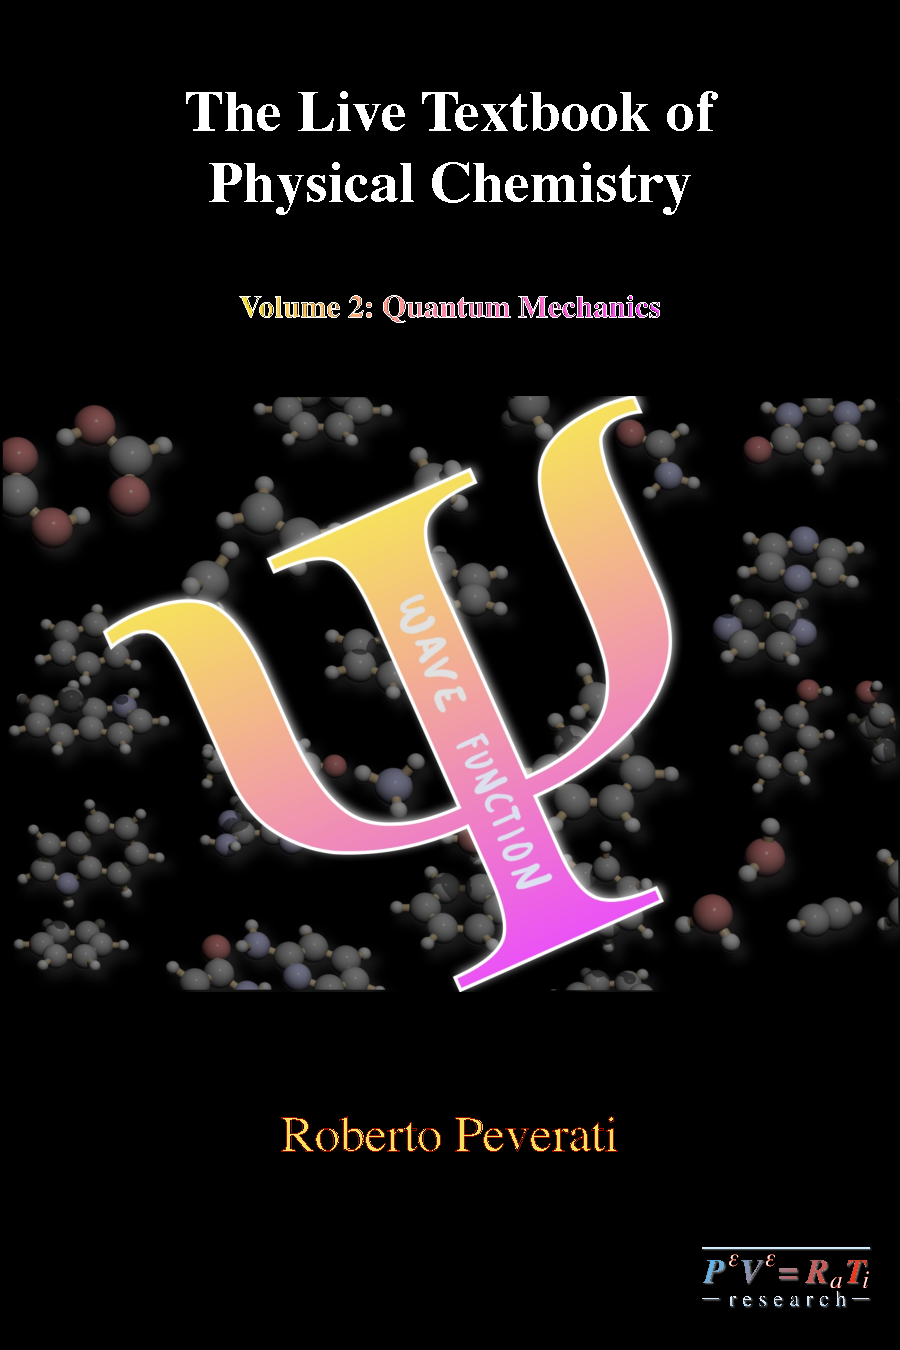
\includepdf[pages={1}, scale=1]{FrontPage_6x9.pdf}
%Frontpage for USLetter:
%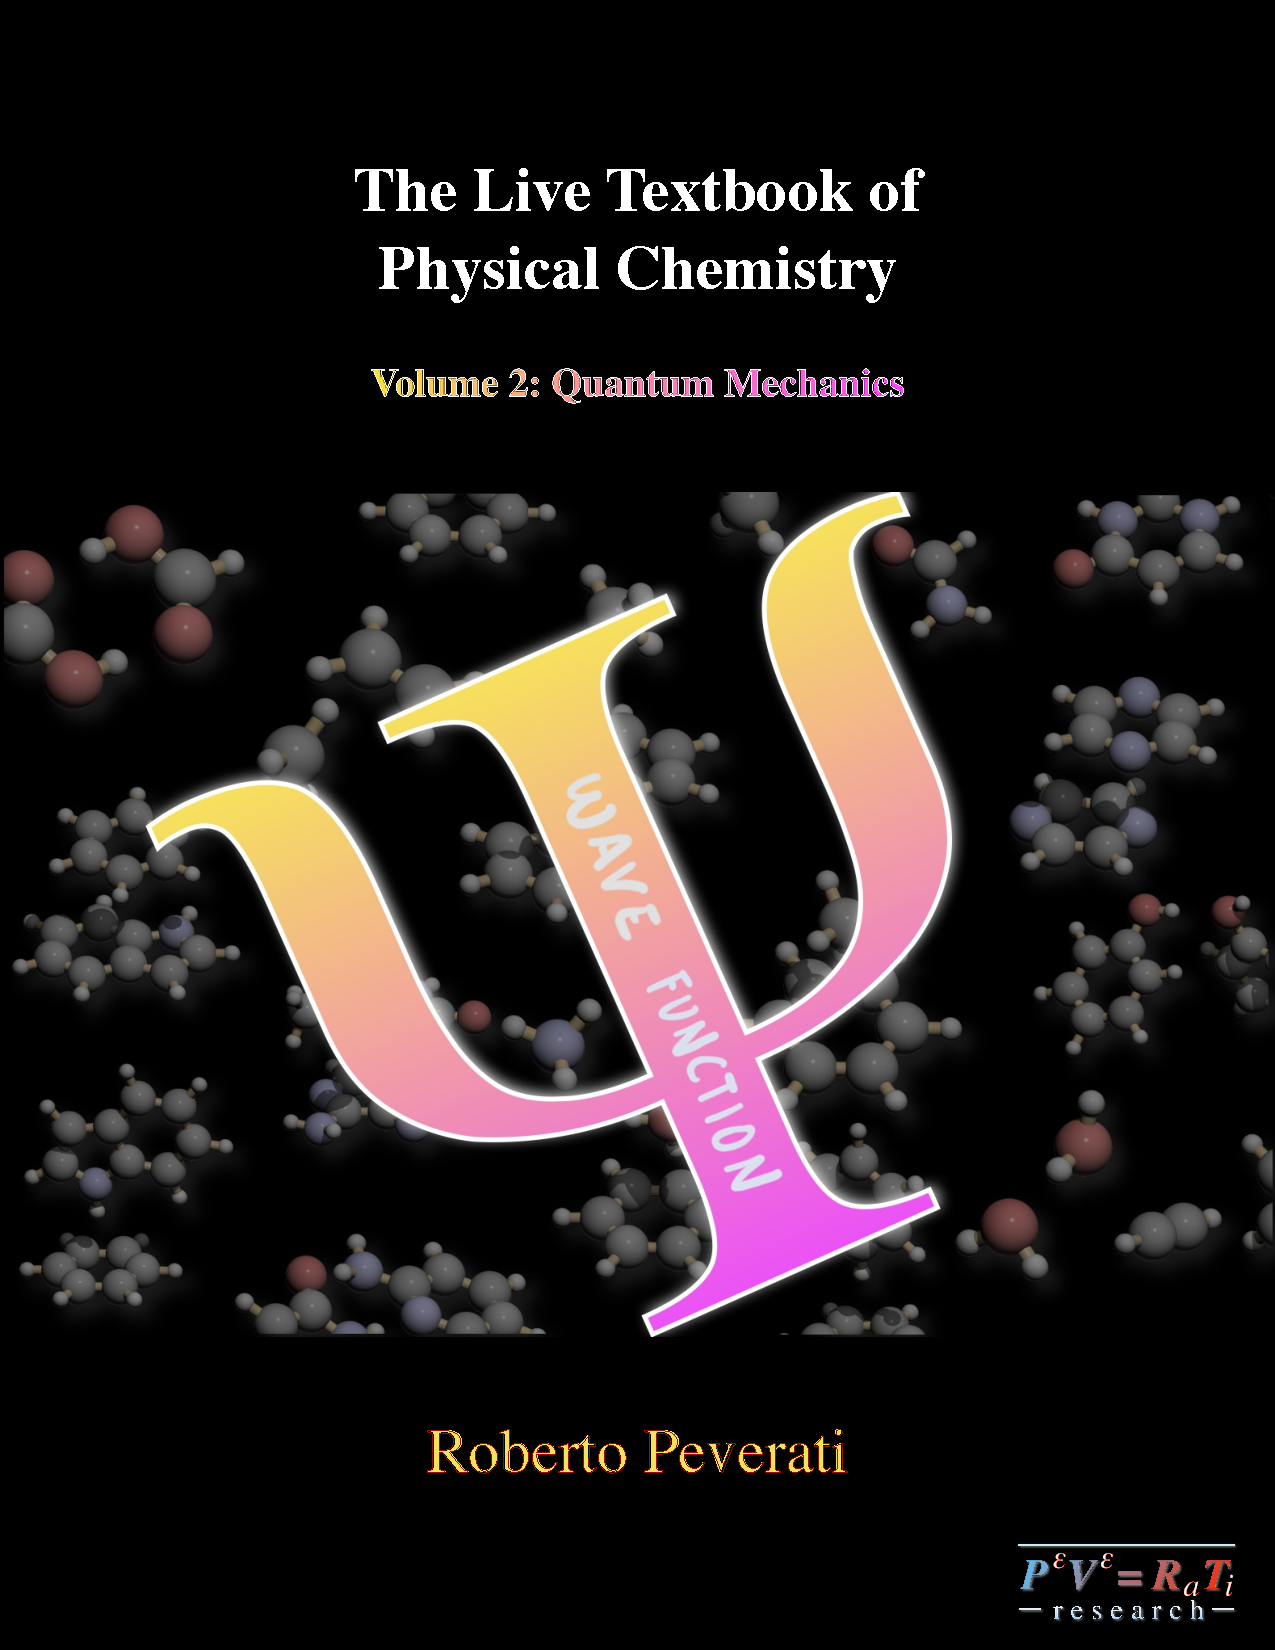
\includepdf[pages={1}, scale=1]{FrontPage.pdf}
\newpage

\let\maketitle\oldmaketitle

% Let's change \thepage so it prints one less than
% the real page number; \pagenumbering{arabic}
% will redefine it to the right meaning afterwards.
\renewcommand\thepage{\romannumeral\numexpr\value{page}-1\relax}


{
\setcounter{tocdepth}{1}
\tableofcontents
}
\renewcommand{\arraystretch}{1.8}

\hypertarget{preface}{%
\chapter*{Preface}\label{preface}}
\addcontentsline{toc}{chapter}{Preface}

\begin{center}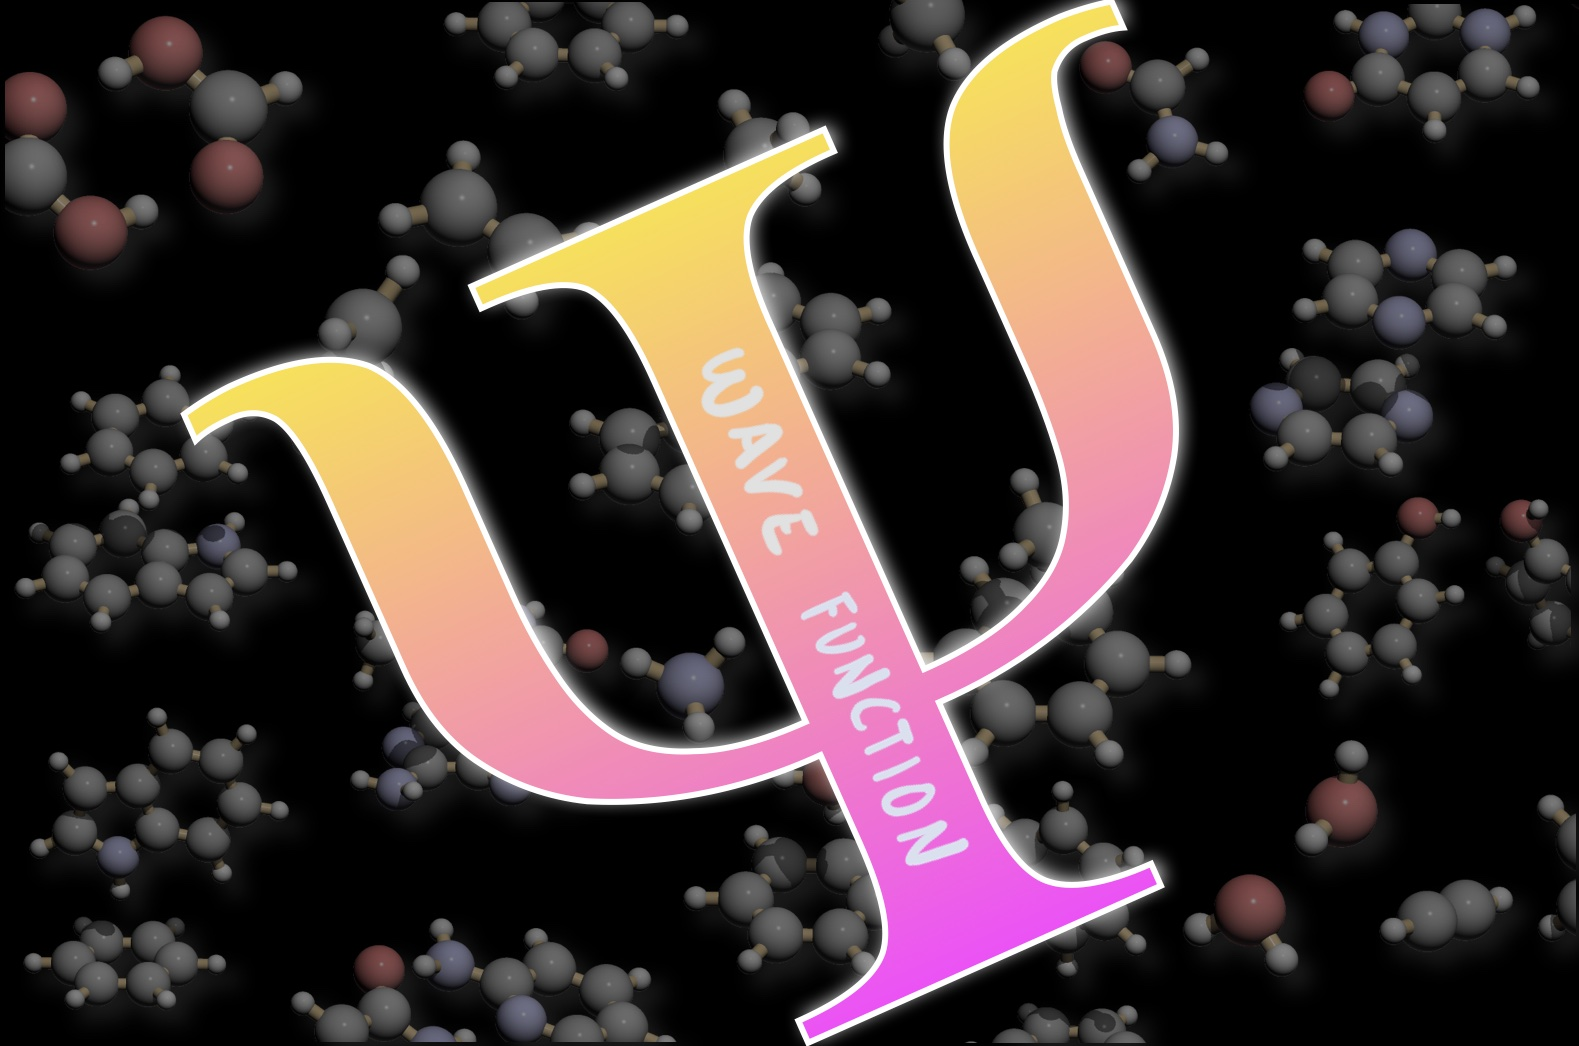
\includegraphics[width=0.8\linewidth]{./img/OEP_Figures.000} \end{center}

This textbook is the official textbook for the Physical Chemistry 2 Course (CHM 3002) at Florida Tech.

The instructor for this course and author of this textbook is Dr.~Roberto Peverati.

\textbf{Contacts}: \href{mailto:rpeverati@fit.edu}{\nolinkurl{rpeverati@fit.edu}}, Office: OPS 333, (321) 674-7735

Chemistry Program, Department of Biomedical and Chemical Engineering and Science
Florida Institute of Technology, Melbourne, FL.

\begin{quote}
This live open textbook is distributed under the \href{https://creativecommons.org/licenses/by-sa/4.0/}{CC-BY-SA 4.0 License} and it was funded by the Florida Tech Open Educational Resources Grant Program: A Collaboration of the Teaching Council, eEducation, and the Evans Library.
\end{quote}

\hypertarget{how-to-use-this-book}{%
\section*{How to use this book}\label{how-to-use-this-book}}
\addcontentsline{toc}{section}{How to use this book}

If you have taken P-Chem 1 at Florida Tech in the Fall Semester 2020, you should already be familiar with this format. Everything we did with the Live Textbook of P-Chem 1 in FS2020 will be happening this semester with P-Chem 2. Please read this book carefully, since everything that will be in your exams is explained here.
Since this book is specifically tailored for the CHM 3002 course at Florida Tech, there are no superfluous parts. In other words, everything in it might be subject to question in the quizzes and the final exam.

\begin{quote}
Definitions and exercises are usually numbered and are highlighted in the text in this format (lighter grey, indented, and following a grey vertical bar). Please study the definitions carefully since they are fundamental concepts that will be used several times in the remainder of the text, and they will be subject to quizzes and exams. Exercises are essential for cementing the concepts, and you should attempt to execute them first without looking at the solution. Even if you were able to solve an exercise on your own, always read the solution after, since it might contain additional explanations expanding the main concepts in the text.
\end{quote}

Navigating the book should be straightforward. On each page, there is a useful sidebar on the left that gives you an overview of all chapters, and a toolbar at the top with important tools. Arrows to shift between chapters might also be present, depending on your browser. If you are old-school and prefer a pdf, you can download a printout by clicking on the toolbar's corresponding icon. If you are \emph{really} old-school and prefer a printed book, the best solution is to download the pdf and print it yourself. It is a LaTeX book, and I can promise you it will look good on paper. However, I cannot provide physical copies to each student. In the toolbar, you will find a useful search box that is capable of searching the entire book. The most adventurous will find in the toolbar a link to the raw GitHub source code. Feel free to head on \href{https://github.com/peverati/PChem2}{over there} and fork the book.

Each chapter of this book represents one week of work in the classroom and at home. The sidebar on the left will reflect your syllabus, as well as the main structure of the class on Canvas. The book is a live document, which means it will be updated throughout the semester with new material. While you are not required to check it every day, you might want to review each week's chapter before the lecture on Friday.

\begin{quote}
If you spot a mistake or a typo, contact Dr.~Peverati via \href{mailto:rpeverati@fit.edu}{email} and you will receive a credit of up to three points towards your final score, once the typo has been verified and corrected.
\end{quote}

\cleardoublepage
\pagenumbering{arabic}

\hypertarget{Motivation}{%
\chapter{The Motivation for Quantum Mechanics}\label{Motivation}}

\hypertarget{introduction}{%
\section{Introduction}\label{introduction}}

Quantum mechanics is an important intellectual achievement of the 20th century. It is one of the more sophisticated field in physics that has affected our understanding of nano-meter length scale systems important for chemistry, materials, optics, and electronics. The existence of orbitals and energy levels in atoms can only be explained by quantum mechanics. Quantum mechanics can explain the behaviors of insulators, conductors, semi-conductors, and giant magneto-resistance. It can explain the quantization of light and its particle nature in addition to its wave nature. Quantum mechanics can also explain the radiation of hot body, and its change of color with respect to temperature. It explains the presence of holes and the transport of holes and electrons in electronic devices.
Quantum mechanics has played an important role in photonics, quantum electronics, and micro-electronics. But many more emerging technologies require the understanding of quantum mechanics; and hence, it is important that scientists and engineers understand quantum mechanics better. One area is nano-technologies due to the recent advent of nano-fabrication techniques. Consequently, nano-meter size systems are more common place. In electronics, as transistor devices become smaller, how the electrons move through the device is quite different from when the devices are bigger: nano-electronic transport is quite different from micro-electronic transport.
The quantization of electromagnetic field is important in the area of nano-optics and quantum optics. It explains how photons interact with atomic systems or materials. It also allows the use of electromagnetic or optical field to carry quantum information. Moreover, quantum mechanics is also needed to understand the interaction of photons with materials in solar cells, as well as many topics in material science.
When two objects are placed close together, they experience a force called the Casimir force that can only be explained by quantum mechanics. This is important for the understanding of micro/nano-electromechanical sensor systems (M/NEMS). Moreover, the understanding of spins is important in spintronics, another emerging technology where giant magneto-resistance, tunneling magneto-resistance, and spin transfer torque are being used.
Quantum mechanics is also giving rise to the areas of quantum information, quantum communication, quantum cryptography, and quantum computing. It is seen that the richness
of quantum physics will greatly affect the future generation technologies in many aspects.

\hypertarget{quantum-mechanics-is-bizarre}{%
\section{Quantum Mechanics is Bizarre}\label{quantum-mechanics-is-bizarre}}

The development of quantum mechanicsis a great intellectual achievement, but at the same time, it is bizarre. The reason is that quantum mechanics is quite different from classical physics. The development of quantum mechanics is likened to watching two players having a game of chess, but the watchers have not a clue as to what the rules of the game are. By observations, and conjectures, finally the rules of the game are outlined. Often, equations are conjectured like conjurors pulling tricks out of a hat to match experimental observations. It is the interpretations of these equations that can be quite bizarre.
Quantum mechanics equations were postulated to explain experimental observations, but the deeper meanings of the equations often confused even the most gifted. Even though Einstein received the Nobel prize for his work on the photo-electric effect that confirmed that light energy is quantized, he himself was not totally at ease with the development of quantum mechanicsas charted by the younger physicists. He was never comfortable with the probabilistic interpretation of quantum mechanics by Born and the Heisenberg uncertainty principle: ``God doesn't play dice,'' was his statement assailing the probabilistic interpretation. He proposed ``hidden variables'' to explain the random nature of many experimental observations. He was thought of as the ``old fool'' by the younger physicists during his time.
Schrödinger came up with the bizarre ``Schrödinger cat paradox'' that showed the struggle that physicists had with quantum mechanics's interpretation. But with today's understanding of quantum mechanics, the paradox is a thing of yesteryear.
The latest twist to the interpretation in quantum mechanics is the parallel universe view that explains the multitude of outcomes of the prediction of quantum mechanics. All outcomes are possible, but with each outcome occurring in different universes that exist in parallel with respect to each other.\footnote{This section was adapted in part from Prof.~Weng Cho CHEW's Quantum Mechanics Made Simple Lecture Notes available \href{http://wcchew.ece.illinois.edu/chew/course/qmall20121005.pdf}{here}.}

The development of quantum mechanics was initially motivated by two observations which demonstrated the inadeqacy of classical physics. These are the ``ultraviolet catastrophe'' and the photoelectric effect.

\hypertarget{the-ultraviolet-catastrophe}{%
\section{The Ultraviolet Catastrophe}\label{the-ultraviolet-catastrophe}}

A blackbody is an idealized object which absorbs and emits all frequencies. Classical physics can be used to derive an equation which describes the intensity of blackbody radiation as a function of frequency for a fixed temperature--the result is known as the Rayleigh-Jeans law. Although the Rayleigh-Jeans law works for low frequencies, it diverges as \(\nu^2\); this divergence for high frequencies is called the ultraviolet catastrophe.
Max Planck explained the blackbody radiation in 1900 by assuming that the energies of the oscillations of electrons which gave rise to the radiation must be proportional to integral multiples of the frequency, i.e.,

\begin{equation}
E = n h \nu
\label{eq:uvcat}
\end{equation}

Using statistical mechanics, Planck derived an equation similar to the Rayleigh-Jeans equation, but with the adjustable parameter \(h\). Planck found that for \(h = 6.626 \times 10^{-34} \; \text{J s}\), the experimental data could be reproduced. Nevertheless, Planck could not offer a good justification for his assumption of energy quantization. Physicicsts did not take this energy quantization idea seriously until Einstein invoked a similar assumption to explain the photoelectric effect.

\hypertarget{the-photoelectric-effect}{%
\section{The Photoelectric Effect}\label{the-photoelectric-effect}}

In 1886 and 1887, Heinrich Hertz discovered that ultraviolet light can cause electrons to be ejected from a metal surface. According to the classical wave theory of light, the intensity of the light determines the amplitude of the wave, and so a greater light intensity should cause the electrons on the metal to oscillate more violently and to be ejected with a greater kinetic energy. In contrast, the experiment showed that the kinetic energy of the ejected electrons depends on the frequency of the light. The light intensity affects only the number of ejected electrons and not their kinetic energies.
Einstein tackled the problem of the photoelectric effect in 1905. Instead of assuming that the electronic oscillators had energies given by Planck's formula, eq. \eqref{eq:uvcat}, Einstein assumed that the radiation itself consisted of packets of energy \(E = h \nu\), which are now called photons. Einstein successfully explained the photoelectric effect using this assumption, and he calculated a value of \(h\) close to that obtained by Planck.

Two years later, Einstein showed that not only is light quantized, but so are atomic vibrations. Classical physics predicts that the molar heat capacity at constant volume (\(C_V\)) of a crystal is \(3 R\), where \(R\) is the molar gas constant. This works well for high temperatures, but for low temperatures \(C_V\) actually falls to zero. Einstein was able to explain this result by assuming that the oscillations of atoms about their equilibrium positions are quantized according to \(E = n h \nu\), Planck's quantization condition for electronic oscillators. This demonstrated that the energy quantization concept was important even for a system of atoms in a crystal, which should be well-modeled by a system of masses and springs (i.e., by classical mechanics).

\hypertarget{wave-particle-duality}{%
\section{Wave-Particle Duality}\label{wave-particle-duality}}

Einstein had shown that the momentum of a photon is

\begin{equation}
p = \frac{h}{\lambda}.
\label{eq:wp1}
\end{equation}

This can be easily shown as follows. Assuming \(E = h \nu\) for a photon and \(\lambda \nu = c\) for an electromagnetic wave, we obtain

\begin{equation}
E = \frac{h c}{\lambda}
\label{eq:wp2}
\end{equation}

Now we use Einstein's relativity result \(E = m c^2\) to find
\begin{equation}
\lambda = \frac{h}{mc}
\label{eq:wp3}
\end{equation}

which is equivalent to eq. \eqref{eq:wp1}. Note that \(m\) refers to the relativistic mass, not the rest mass, since the rest mass of a photon is zero. Since light can behave both as a wave (it can be diffracted, and it has a wavelength), and as a particle (it contains packets of energy \(h \nu\)), de Broglie reasoned in 1924 that matter also can exhibit this wave-particle duality. He further reasoned that matter would obey the same eq. \eqref{eq:wp1} as light. In 1927, Davisson and Germer observed diffraction patterns by bombarding metals with electrons, confirming de Broglie's proposition.\footnote{The previous 3 sections were adapted in part from Prof.~C. David Sherrill's A Brief Review of Elementary Quantum Chemistry Notes available \href{http://vergil.chemistry.gatech.edu/notes/quantrev/node1.html}{here}.}

Rewriting the previous equations in terms of the wave vector, \(k=\frac{2\pi}{\lambda}\), and the angular frequency, \(\omega=2\pi\nu\), we obtain the following two equations

\begin{equation}
\begin{aligned}
p &= \hbar k \\
E &= \hbar \omega,
\end{aligned}
\label{eq:wp1b}
\end{equation}

which are known as \textbf{de Broglie's equations}. We will use those equation to develop wave mechanics in the next chapters.

\hypertarget{Classical}{%
\chapter{Classical Mechanics}\label{Classical}}

Quantum mechanics cannot be derived from classical mechanics, but classical mechanics can inspire quantum mechanics. Quantum mechanics is richer and more sophisticated than classical mechanics. Quantum mechanics was developed during the period when physicists had rich knowledge of classical mechanics. In order to better understand how quantum mechanics was developed in this envirgonment, it is better to understand some fundamental concepts in classical mechanics. Classical mechanics can be considered as a special case of quantum mechanics. We will review some classical mechanics concepts here.

\hypertarget{newtonian-formulation}{%
\section{Newtonian Formulation}\label{newtonian-formulation}}

In classical mechanics, a particle moving in the presence of potential \(V(q)\) will experience a force given by:

\begin{equation}
F(q) = -\frac{dV(q)}{dq},
\label{eq:class1}
\end{equation}

where \(q\) represents the coordinate or the position of the particle. Hence, the particle can be described by the equations of motion:

\begin{equation}
\frac{dp}{dt} = F(q) = -\frac{dV (q)}{dq},\quad \frac{dq}{dt} = \frac{p}{m}.
\label{eq:class2}
\end{equation}

For example, when a particle is attached to a spring and moves along a frictionless surface, the force the particle experiences is \(F(q) = -kq\) where \(k\) is the spring constant. Then the equations of motion of this particle are

\begin{equation}
\frac{dp}{dt} =\dot{p}=-kq,\quad \frac{dq}{dt} =\dot{q}=p/m
\label{eq:class3}
\end{equation}

Given \(p\) and \(q\) at some initial time \(t_0\), one can integrate \eqref{eq:class2} or \eqref{eq:class3} to obtain \(p\) and \(q\) for all later time. Notice that only two variables \(p\) and \(q\) are sufficient to describe the state of a particle. These equations of motion are essentially derived using Newton's law. However, there are at least two other methods of deriving these equations of motion, which are described below.

\hypertarget{lagrangian-formulation}{%
\section{Lagrangian Formulation}\label{lagrangian-formulation}}

Another way to derive the equations of motion for classical mechanics is via the use of the Lagrangian and the principle of least action. The Lagrangian formulation is obtained by starting from the definition of the Lagrangian of the system:

\begin{equation}
L = K - V,
\label{eq:lag1}
\end{equation}

where \(K\) is the kinetic energy, and \(V\) is the potential energy. Both are expressed in terms of coordinates \((q,\dot{q}\)) where \(q\) \(\in\) \(\mathbb{R}^{n}\) is the position vector and \(\dot{q}\) \(\in\) \(\mathbb{R}^{n}\) is the velocity vector. Notice that for a fixed time, \(t\), \(q\) and \(\dot{q}\) are independent variables, since \(\dot{q}\) cannot be derived from \(q\) alone.

The time integral of the Lagrangian is called the \textbf{action}, and is defined as:

\begin{equation}
S = \int_{t_1}^{t_2} L\, dt,
\label{eq:lag2}
\end{equation}

which is a functional: it takes in the Lagrangian function for all times between \(t_1\) and \(t_2\) and returns a scalar value. The equations of motion can be derived from the principle of least action,\footnote{Sometimes also called principle of stationary action, or variational principle, or Hamilton's principle.} which states that the true evolution of a system \(q(t)\) described by the coordinate \(q\) between two specified states \(q_1 = q(t_1)\) and \(q_2 = q(t_2)\) at two specified times \(t_1\) and \(t_2\) is a stationary point of the action functional. For a stationary point:

\begin{equation}
\delta     S = \frac{dS}{dq}= 0
\label{eq:lag3}
\end{equation}

Requiring that the true trajectory \(q(t)\) be a stationary point of the action functional \(S\) we obtain the equation of motion (figure \ref{fig:Fig1c2}\^{}{[}This diagram is taken from \href{https://en.wikipedia.org}{Wikipedia} by user Maschen, and distributed under CC0 license). This can be achieved applying classical variational calculus to the variation of the action integral \(S\) under perturbations of the path \(q(t)\) (eq. \eqref{eq:lag3}). The resulting equation of motion (or set of equations in the case of many dimensions) is sometimes also called the Euler---Lagrange equation:\footnote{The mathematical derivation of the Euler---Lagrange equaiton is rather long and unimportant at this stage. For the curious, it can be found \href{https://en.wikipedia.org/wiki/Euler–Lagrange_equation}{here}.}

\begin{equation}
\frac{d}{dt}\left(\frac{\partial L}{\partial\dot q}\right)=\frac{\partial L}{\partial q}.
\label{eq:lag4}
\end{equation}

\begin{figure}

{\centering 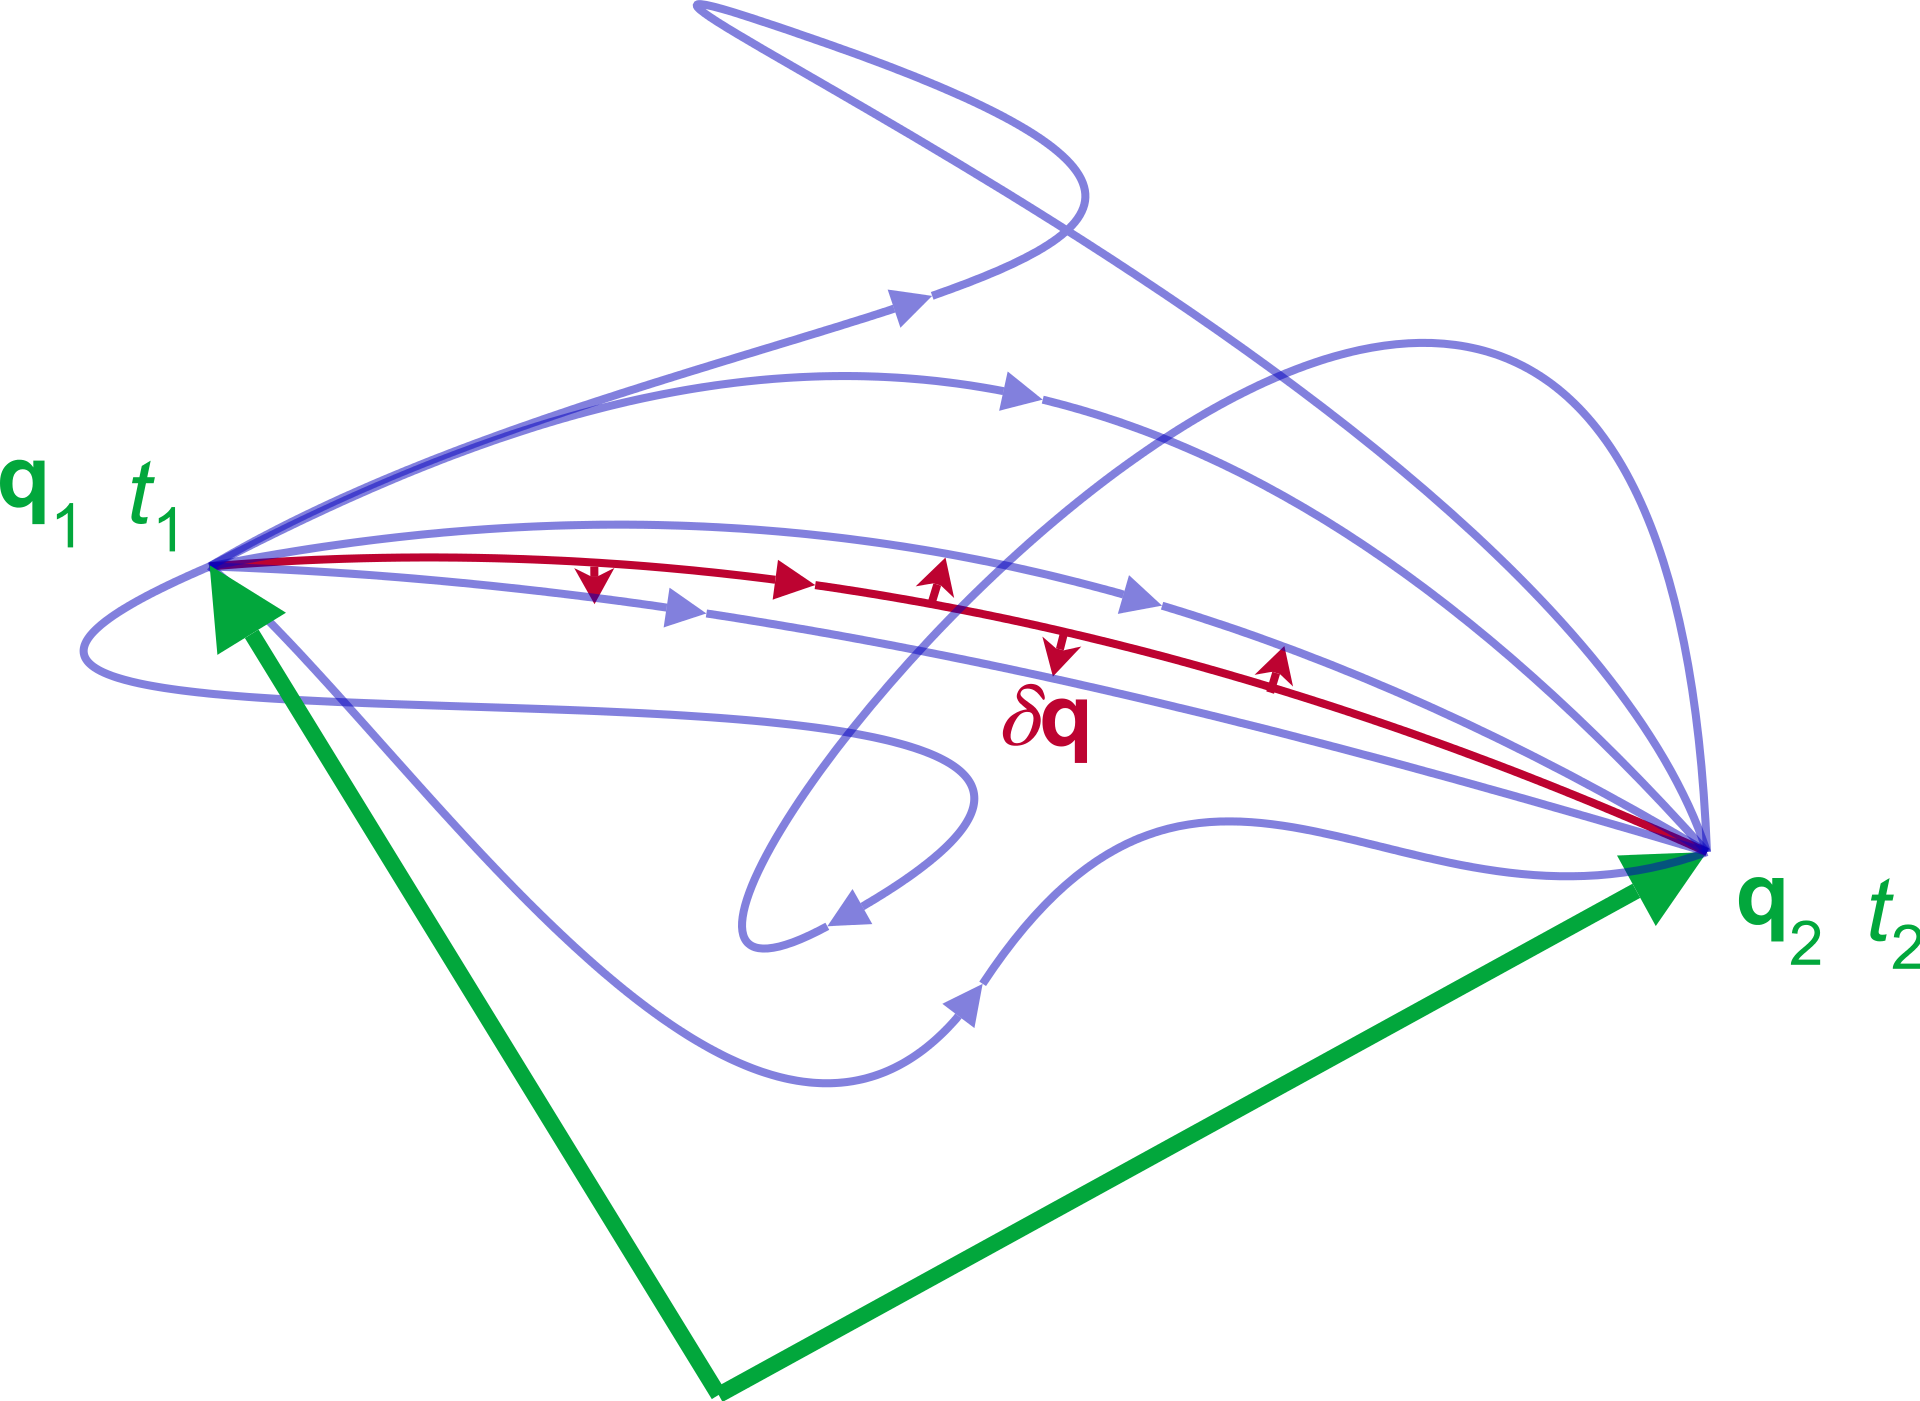
\includegraphics[width=0.7\linewidth]{./img/OEP_wiki1} 

}

\caption{Principle of least action: As the system evolves, q traces a path through configuration space (only some are shown). The path taken by the system (red) has a stationary action under small changes in the configuration of the system.}\label{fig:Fig1c2}
\end{figure}

\hypertarget{hamiltonian-mechanics}{%
\section{Hamiltonian mechanics}\label{hamiltonian-mechanics}}

A third way of obtaining the equation of motion is Hamiltonian mechanics, which uses the generalized momentum in place of velocity as a coordinate. The generalized momentum is defined in terms of the Lagrangian and the coordinates \((q,\dot{q})\):

\begin{equation} 
p = \frac{\partial L}{\partial\dot q}.
\label{eq:ham1}
\end{equation}

The Hamiltonian is defined from the Lagrangian by applying a Legendre transformation as:\footnote{We have already encountered Legendre transform in \href{https://peverati.github.io/pchem1/Potentials.html\#thermpot}{The Live Textbook of Physical Chemistry 1} when transforming from the thermodynamic energy to any of the other thermodynamic potentials.}

\begin{equation} 
H(p,q) = p\dot{q} - L(q,\dot{q}),
\label{eq:ham2}
\end{equation}

The Lagrangian equation of motion becomes a pair of equations known as the Hamiltonian system of equations:

\begin{equation} 
\begin{aligned}
\dot{p}=\frac{dp}{dt} &= -\frac{\partial H}{\partial q} \\
\dot{q}=\frac{dq}{dt} &= +\frac{\partial H}{\partial p},
\end{aligned}
\label{eq:ham3}
\end{equation}

where \(H=H(q,p,t)\) is the Hamiltonian of the system, which often corresponds to its total energy. For a closed system, it is the sum of the kinetic and potential energy in the system:

\begin{equation}
H = K + V.
\label{eq:hamdef}
\end{equation}

Notice the difference between the Hamiltonian, eq. \eqref{eq:hamdef}, and the Lagrangian, eq. \eqref{eq:lag1}. In Newtonian mechanics, the time evolution is obtained by computing the total force being exerted on each particle of the system, and from Newton's second law, the time evolutions of both position and velocity are computed. In contrast, in Hamiltonian mechanics, the time evolution is obtained by computing the Hamiltonian of the system in the generalized momenta and inserting it into Hamilton's equations. This approach is equivalent to the one used in Lagrangian mechanics, since the Hamiltonian is the Legendre transform of the Lagrangian. The main motivation to use Hamiltonian mechanics instead of Lagrangian mechanics comes from the more simple description of complex dynamic systems.

\begin{quote}
\begin{example}
\protect\hypertarget{exm:hamex1}{}{\label{exm:hamex1} }\emph{Basic Interpretation of Hamiltonian Mechanics}

A simple interpretation of Hamiltonian mechanics comes from its application on a one-dimensional system consisting of one particle of mass \(m\). The Hamiltonian can represent the total energy of the system, which is the sum of kinetic and potential energy.

\begin{equation}
\begin{aligned}
H &= K+V \\
K &={\frac {p^{2}}{2m}},\quad V=V(q),
\end{aligned}
\label{eq:ham4}
\end{equation}

where \(q\) is the space coordinate and \(p=m\dot{q}\) is the momentum. Then
\(k\) is a function of \(p\) alone, while \(V\) is a function of \(q\) alone.

In this example, the time derivative of the momentum \(p\) equals the Newtonian force, and so the first Hamilton equation means that the force equals the negative gradient of potential energy:

\begin{equation}
\text{Newtonian force:}\qquad \frac{dp}{dt} = -\frac{\partial V(q)}{\partial q},
\label{eq:ham5}
\end{equation}

which is exactly the first equation of motion in eq. \eqref{eq:class2} of Newtonian mechanics. Notice that this equaiton could have been easily obtained in the Lagrangian formulation by writing the Lagrangian \eqref{eq:lag1}, and using the Euler-Lagrange equation, eq. \eqref{eq:lag4}.
The time derivative of \(q\) is the velocity, and so the second Hamilton equation means that the particle's velocity equals the derivative of its kinetic energy with respect to its momentum:

\begin{equation}
\text{Velocity:}\qquad \frac{dq}{dt} = \frac{\partial K}{\partial p} = \frac{\partial \left(\frac{p^2}{2m}\right)}{\partial p} = \frac{p}{m},
\label{eq:ham6}
\end{equation}

which is exactly the second equation of motion in eq. \eqref{eq:class2} of Newtonian mechanics.
\end{example}
\end{quote}

\hypertarget{Schrodinger}{%
\chapter{The Schrödinger Equation}\label{Schrodinger}}

In 1925, Erwin Schrödinger and Werner Heisenberg independently developed the new quantum theory. Schrödinger's method involves partial differential equations, whereas Heisenberg's method employs matrices; however, a year later the two methods were shown to be mathematically equivalent. Most textbooks begin with Schrödinger's equation, since it seems to have a better physical interpretation via the classical wave equation. Indeed, the Schrödinger equation can be viewed as a form of the wave equation applied to matter waves.

\hypertarget{the-time-independent-schruxf6dinger-equation}{%
\section{The Time-Independent Schrödinger Equation}\label{the-time-independent-schruxf6dinger-equation}}

We can start the derivation of the single-particle time-independent Schrödinger equation (TISEq) from the equation that describes the motion of a wave in classical mechanics:

\begin{equation}
\psi(x,t)=\exp[i(kx-\omega t)],
\label{eq:sch1}
\end{equation}

where \(x\) is the position, \(t\) is time, \(k=\frac{2\pi}{\lambda}\) is the wave vector, and \(\omega=2\pi\nu\) is the angular frequency of the wave. If we are not concerned with the time evolution, we can consider uniquely the derivatives of eq. \eqref{eq:sch1} with respect to the location, which are:

\begin{equation}
\begin{aligned}
\frac{\partial \psi}{\partial x} &=ik\exp[i(kx-\omega t)] = ik\psi, \\
\frac{\partial^2 \psi}{\partial x^2} &=i^2k^2\exp[i(kx-\omega t)] = -k^2\psi,
\end{aligned}
\label{eq:sch2}
\end{equation}

where we have used the fact that \(i^2=-1\).

Assuming that particles behaves as wave---as proven by de Broglie's we can now use the first of de Broglie's equation, eq. \eqref{eq:wp1b}, we can replace \(k=\frac{p}/{\hbar}\) to obtain:

\begin{equation}
\frac{\partial^2 \psi}{\partial x^2} = -\frac{p^2\psi}{\hbar^2},
\label{eq:sch3}
\end{equation}

which can be rearranged to:

\begin{equation}
p^2 \psi = -\hbar^2 \frac{\partial^2 \psi}{\partial x^2}.
\label{eq:sch4}
\end{equation}

The total energy associated with a wave moving in space is simply the sum of its kinetic and potential energies:

\begin{equation}
E = \frac {p^{2}}{2m} + V(x),
\label{eq:sch5}
\end{equation}

from which we can obtain:

\begin{equation}
p^2 = 2m[E - V(x)],
\label{eq:sch6}
\end{equation}

which we can then replace into eq. \eqref{eq:sch4} to obtain:

\begin{equation}
2m[E-V(x)]\psi = - \hbar^2 \frac{\partial^2 \psi}{\partial x^2},
\label{eq:sch7}
\end{equation}

which can then be rearranged to the famous \textbf{time-independent Schrödinger equation (TISEq)}:

\begin{equation}
- \frac{\hbar^2}{2m} \frac{\partial^2 \psi}{\partial x^2} + V(x) \psi = E\psi,
\label{eq:TISEq}
\end{equation}

A two-body problem can also be treated by this equation if the mass \(m\) is replaced with a reduced mass \(\mu = \frac{m_1 m_2}{m_1+m_2}\).

\hypertarget{the-time-dependent-schruxf6dinger-equation}{%
\section{The Time-Dependent Schrödinger Equation}\label{the-time-dependent-schruxf6dinger-equation}}

Unfortunately, the analogy with the classical wave equation that allowed us to obtain the TISEq in the previous section cannot be extended to the time domain by considering the equation that involves the partial first derivative with respect to time. Schrödinger himself presented his time-independent equation first, and then went back and postulated the more general time-dependent equation. We are following here the same strategy and just give the time-independent variable as a postulate. The single-particle time-dependent Schrödinger equation is:

\begin{equation}
i\hbar\frac{\partial \psi(x,t)}{\partial t}=-\frac{\hbar^2}{2m} \frac{\partial^2 \psi(x,t)}{\partial x^2}+V(x)\psi(x,t)
\label{eq:TDSEq}
\end{equation}

where \(V \in \mathbb{R}^{n}\) represents the potential energy of the system.
Obviously, the time-dependent equation can be used to derive the time-independent equation. If we write the wavefunction as a product of spatial and temporal terms, \(\psi(x, t) = \psi(x) f(t)\), then equation \eqref{eq:TDSEq} becomes:

\begin{equation}
\psi(x) i \hbar \frac{df(t)}{dt} = f(t) \left[-\frac{\hbar^2}{2m} \frac{\partial^2}{\partial x^2} + V(x) \right] \psi(x),
\label{eq:TDSEq2}
\end{equation}

which can be rearranged to:

\begin{equation}
\frac{i \hbar}{f(t)} \frac{df(t)}{dt} = \frac{1}{\psi(x)} \left[-\frac{\hbar^2}{2m} \frac{\partial^2}{\partial x^2} + V(x) \right] \psi(x).
\label{eq:TDSEq3}
\end{equation}

Since the left-hand side of eq. \eqref{eq:TDSEq3} is a function of \(t\) only and the right hand side is a function of \(x\) only, the two sides must equal a constant. If we tentatively designate this constant \(E\) (since the right-hand side clearly must have the dimensions of energy), then we extract two ordinary differential equations, namely:

\begin{equation}
\frac{1}{f(t)} \frac{df(t)}{dt} = - \frac{i E}{\hbar}
\label{eq:TDSEq4}
\end{equation}

and:
\begin{equation}
-\frac{\hbar^2}{2m} \frac{\partial^2\psi(x)}{\partial x^2} + V(x) \psi(x) =
E \psi(x).
\label{eq:TDSEq5}
\end{equation}

The latter equation is the TISEq. The former equation is easily solved to yield

\begin{equation}
f(t) = e^{-iEt / \hbar}
\label{eq:TDSEq6}
\end{equation}

The solutions of eq. \eqref{eq:TDSEq6}, \(f(t)\), are purely oscillatory, since \(f(t)\) never changes in magnitude. Thus if:

\begin{equation}
\psi(x, t) = \psi(x) \exp\left(\frac{-iEt}{\hbar}\right),
\label{eq:TDSEq6b}
\end{equation}

then the total wave function \(\psi(x, t)\) differs from \(\psi(x)\) only by a phase factor of constant magnitude. There are some interesting consequences of this. First of all, the quantity \(\vert \psi(x, t) \vert^2\) is time independent, as we can easily show:

\begin{equation}
\vert \psi(x, t) \vert^2 = \psi^{*}(x, t) \psi(x, t)=
\exp\left(\frac{iEt}{\hbar}\right)\exp\left(\frac{-iEt}{\hbar}\right)=
\psi^{*}(x) \psi(x).
\label{eq:TDSEq7}
\end{equation}

Wave functions of the form of eq. \eqref{eq:TDSEq6b} are called stationary states. The state \(\psi(x, t)\) is ``stationary,'' but the particle it describes is not!
Of course eq. \eqref{eq:TDSEq6} represents only a particular solution to the time-dependent Schrödinger equation. The general solution is, in general, much more complicated.\footnote{This sections was adapted in part from Prof.~C. David Sherrill's A Brief Review of Elementary Quantum Chemistry Notes available \href{http://vergil.chemistry.gatech.edu/notes/quantrev/node1.html}{here}.}

\begin{equation}
\psi({\bf r}, t) = \sum_i c_i e^{-iE_it / \hbar} \psi_i({\bf r})
\end{equation}

\hypertarget{Models}{%
\chapter{Analytically Soluble Models}\label{Models}}

The TISEq can be solved analytically only in a few special cases. In this section, we will analyze the main four. Luckily, we can use these solutions to explain most of the effects in chemistry since we can combine them to describe the hydrogen atom upon which we can build more complex chemical systems, as we will show in the next chapters.

\hypertarget{the-free-particle}{%
\section{The Free Particle}\label{the-free-particle}}

By definition, the particle does not feel any external force, therefore \(V(x)=0\), and the TISEq is written simply:

\begin{equation}
- \frac{\hbar^2}{2m} \frac{d^2\psi}{dx^2} = E \psi(x).
\label{eq:FP1}
\end{equation}

This equation can be rearranged to:

\begin{equation}
\frac{d^2\psi}{dx^2} =- \frac{2mE}{\hbar^2} \psi(x),
\label{eq:FP2}
\end{equation}

which corresponds to a mathematical problem where the second derivative of a function should be equal to a constant, \(- \frac{2mE}{\hbar^2}\) multiplied by the function itself. Such a problem is easily solved by the function:

\begin{equation}
\psi(x) = A \exp(\pm ikx).
\label{eq:FP3}
\end{equation}

The first and second derivatives of this function are:

\begin{equation}
\begin{aligned}
\frac{d \psi(x)}{dx} &= \pm ik A \exp(\pm ikx) = \pm ik \psi(x) \\
\frac{d^2 \psi(x)}{dx^2} &= \mp k^2  A \exp(\pm ikx) = -(\pm k^2) \psi(x). 
\end{aligned}
\label{eq:FP4}
\end{equation}

Comparing the second derivative in eq. \eqref{eq:FP4} with eq. \eqref{eq:FP2}, we immediately see that if we set:

\begin{equation}
k^2 = \frac{2mE}{\hbar^2},
\label{eq:FP5}
\end{equation}

we solve the original differential equation. Considering de Broglie's equation, eq. \eqref{eq:wp1b}, we can replace \(k=\frac{p}{\hbar}\), to obtain:

\begin{equation}
E = \frac{k^2 \hbar^2}{2m} = \frac{p^2}{2m},
\label{eq:FP6}
\end{equation}

which is exactly the classical value of the kinetic energy of a free particle moving in one direction of space. Since the function in eq. \eqref{eq:FP3} solves the Schrödinger equation for the free particle, it is called an \emph{eigenfunction} (or \emph{eigenstate}) of the TISEq. The energy result of eq. \eqref{eq:FP6} is called \emph{eigenvalue} of the TISEq. Notice that, since \(k\) is continuous in the eigenfunction, the energy eigenvalue is also continuous (i.e., all values of \(E\) are acceptable).

\hypertarget{rigidrotor}{%
\section{The Particle in a Box}\label{rigidrotor}}

Now we can consider a particle constrained to move in a single dimension, under the influence of a potential \(V(x)\) which is zero for \(0 \leq x \leq a\) and infinite elsewhere. Since the wavefunction is not allowed to become infinite, it must have a value of zero where \(V(x)\) is infinite, so \(\psi(x)\) is nonzero only within \([0,a]\). The Schrödinger equation is thus:

\begin{equation}
- \frac{\hbar^2}{2m} \frac{d^2\psi}{dx^2} = E \psi(x)
\qquad 0 \leq x \leq a.
\label{eq:PIB1}
\end{equation}

In other words, inside the box \(\psi(x)\) describes a free particle, but outside the box \(\psi(x)=0\). Since the Schrödinger equation involves derivatives, the function that solves it, \(\psi(x)\), must be everywhere continuous and everywhere continuously differentiable. This fact means that the value of the wave function at the two extremes must be equal to zero:

\begin{equation}
\psi(0)=\psi(a)=0.
\label{eq:PIB2}
\end{equation}

Inside the box we can use Euler's formula to write the wave function as a linear combination of the positive and negative solutions:

\begin{equation}
\psi(x)=A \exp(\pm ix)=A \sin kx + B \cos kx,
\label{eq:PIB3}
\end{equation}

where \(A\) and \(B\) are constants that we need to determine using the two constraints in eq. \eqref{eq:PIB2}. For \(B\) it is straightforward to see that:

\begin{equation}
\psi(0)= 0 + B =0 \; \implies \; B=0.
\label{eq:PIB4}
\end{equation}

For \(A\) we have:

\begin{equation}
\psi(a)= A\sin ka = 0,
\label{eq:PIB5}
\end{equation}

which is trivially solved by \(A=0\), or by the more interesting condition of \(ka=n\pi\). The trivial solution corresponds to a wave function uniformly equal to zero everywhere. This wave function is uninteresting, since it describes no particles in no boxes. The second set of solutions, however, is very interesting, since we can write it as:

\begin{equation}
\psi_n(x)= A\sin\left(\frac{n\pi x}{a} \right)\quad n=1,2,\ldots,\infty,
\label{eq:PIB6}
\end{equation}

which represents an infinite set of functions, \(\psi_n(x)\), determined by a positive integer number \(n\), called \emph{qunatum number}. Since these functions solve the TISEq, they are also called \emph{eigenfunctions}, but they are not a continuous set, unlike in the previous case. To calculate the energy eigenvalues, we can replace \eqref{eq:PIB6} into eq. \eqref{eq:PIB1}, to obtain:

\begin{equation}
E_n = \frac{h^2 n^2}{8 m a^2} \quad n=1,2,\ldots,\infty.
\label{eq:PIB7}
\end{equation}

A few interesting considerations can be made from the results of eq. \eqref{eq:PIB7}. First, although there is an infinite number of acceptable values of the energy (eigenvalues), these values are not continuous. Second, the lowest value of the energy is not zero, and it depends on the size of the box, \(a\), since:

\begin{equation}
E_1 = \frac{h^2 }{8 m a^2} \neq 0.
\label{eq:PIB8}
\end{equation}

This value is called \emph{zero-point energy (ZPE)}, and is a purely quantum mechanical effect. Notice that we did not solve for the constant \(A\). This task is not straightforward, and it can be achieved by requiring the wave function to describe one particle exclusively (we will come back to this task after chapter 7). Extending the problem to three dimensions is relatively straightforward, resulting in a set of three separate quantum numbers (one for each of the 3-dimensional coordinate \(n_x,n_y,n_z\)).

\hypertarget{the-harmonic-oscillator}{%
\section{The Harmonic Oscillator}\label{the-harmonic-oscillator}}

We now consider a particle subject to a restoring force \(F = -kx\), as might arise for a mass-spring system obeying Hooke's Law. The potential is then:

\begin{equation}
V(x) = - \int_{-\infty}^{\infty} (-kx) dx = V_0 + \frac{1}{2} kx^2.
\label{eq:HO1}
\end{equation}

If we choose the energy scale such that \(V_0 = 0\) then: \(V(x) = (1/2)kx^2\), and the TISEq looks:

\begin{equation}
- \frac{\hbar^2}{2 \mu} \frac{d^2\psi}{dx^2} + \frac{1}{2} kx^2 \psi(x) =
E \psi(x)
\label{eq:HO2}
\end{equation}

After some effort, the eigenfunctions are:

\begin{equation}
\psi_n(x) = N_n H_n(\alpha^{1/2} x) e^{-\alpha x^2 / 2} \quad n=0,1,2,\ldots,\infty,
\label{eq:HO3}
\end{equation}

where \(H_n\) is the Hermite polynomial of degree \(n\), and \(\alpha\) and \(N_n\) are defined by

\begin{equation}
\alpha = \sqrt{\frac{k \mu}{\hbar^2}} \hspace{1.5cm}
N_n = \frac{1}{\sqrt{2^n n!}} \left( \frac{\alpha}{\pi} \right)^{1/4}.
\label{eq:HO4}
\end{equation}

The eigenvalues are:

\begin{equation}
E_n = \hbar \omega (n + \frac{1}{2}),
\label{eq:HO5}
\end{equation}

with \(\omega = \sqrt{k/ \mu}\). Notice how, once again, the eigenfunctions and eigenvalues are not continuous. In this case, however, the first eigenvalue corresponds to \(n=0\), but because of the \(\frac{1}{2}\) factor in eq. \eqref{eq:HO5}, the lowest energy state is, once again, not zero. In other words, the two masses of a quantum harmonic oscillator are always in motion. The frequencies at which they vibrate do not form a continuous spectrum. That is, the vibration frequency cannot take any value that we can think of, but only those given by eq. \eqref{eq:HO5}. The lowest possible energy (the ZPE) will be \(E_0 = \frac{1}{2} \hbar \omega\).

\hypertarget{the-rigid-rotor}{%
\section{The Rigid Rotor}\label{the-rigid-rotor}}

The rigid rotor is a simple model of a rotating stick in three dimensions (or, if you prefer, of a molecule). We consider the stick to consist of two point-masses at a fixed distance. We then reduce the model to a one-dimensional system by considering the rigid rotor to have one mass fixed at the origin, which is orbited by the reduced mass \(\mu\), at a distance \(r\). The cartesian coordinates, \(x,y,z\), are then replaced by three spherical polar coordinates: the co-latitude (zenith) angle \(\theta\), the longitudinal (azimuth) angle \(\phi\), and the distance \(r\). The TISEq of the system in spherical coordinates is:

\begin{equation}
- \frac{\hbar^2}{2I} \left[ \frac{1}{\sin \theta}
\frac{\partial}{\partial \theta} \left(\sin\theta\frac{\partial}{\partial \theta} \right) + \frac{1}{\sin^2 \theta} \frac{\partial^2}{\partial \phi^2} \right] \psi(r) = E \psi(r),
\label{eq:RR1}
\end{equation}

where \(I=\mu r^2\) is the moment of inertia. After a little effort, the eigenfunctions can be shown to be the spherical harmonics \(Y_{\ell}^m(\theta, \phi)\).\footnote{For a description of the spherical harmonics see \href{https://en.wikipedia.org/wiki/Spherical_harmonic}{here}} The eigenvalues are simply:

\begin{equation}
E_{\ell} = \frac{\hbar^2}{2I} \ell(\ell+1).
\label{eq:RR2}
\end{equation}

Each energy level \(E_{\ell}\) is \(2\ell+1\)-fold degenerate in \(m\), since \(m\) can have values \(-\ell, -\ell+1, \ldots, \ell-1, \ell\). Notice also that the energy does not depend on the second index \(m\), and the functions with fixed \(m=-\ell,-\ell+1,\dots,\ell-1,\ell\) have the same energy. Since this problem was, in fact, a one-dimensional problem, it results in just one quantum number \(\ell\), similarly to the previous two cases. The index \(m\) that appears in the spherical harmonics will assume some importance in future chapters.

\hypertarget{Hydrogen}{%
\chapter{The Hydrogen Atom}\label{Hydrogen}}

In this chapter we will consider the hydrogen atom as a proton fixed at the origin, orbited by an electron of reduced mass \(\mu\). The potential due to electrostatic attraction is:

\begin{equation}
V(r) = - \frac{e^2}{4 \pi \varepsilon_0 r},
\label{eq:HA1}
\end{equation}

where \(\varepsilon_0\) is the constant permittivity of vacuum.
The kinetic energy term in the Hamiltonian is

\begin{equation}
K = - \frac{\hbar^2}{2 \mu} \nabla^2,
\label{eq:HA2}
\end{equation}

where \(\nabla^2\) is the Laplace operator (\emph{Laplacian}) representing the divergence of the gradient of a function. Recall that in 1-dimension the kinetic energy is proportional to the second derivative of the wave function with respect to the position. In 3-dimension, the dirst derivative along all three dimension of space is called gradient, which is written in cartesian coordinates \(\nabla = \left(\frac{\partial}{\partial x},\frac{\partial}{\partial y},\frac{\partial}{\partial z} \right)\). The Laplacian is the divergence \(\nabla \cdot\) of the gradient (effectively, it replaces the second derivatives in the 1-D case), and can be written in cartesian coordinates as \(\nabla\cdot\nabla=\nabla^2=\frac{\partial^2}{\partial x^2}+\frac{\partial^2}{\partial y^2},\frac{\partial^2}{\partial z^2}\). The TISEq for the Hydrogen atom is therefore:

\begin{equation}
{\displaystyle \left(-{\frac {\hbar ^{2}}{2\mu }}\nabla ^{2}-{\frac {e^{2}}{4\pi \varepsilon _{0}r}}\right)\psi (r,\theta ,\phi )=E\psi (r,\theta ,\phi )},
\label{eq:HA2b}
\end{equation}

which, replacing the Laplacian in spherical coordinates, becomes:

\begin{equation}
-{\frac {\hbar ^{2}}{2\mu }}\left[{\frac {1}{r^{2}}}{\frac {\partial }{\partial r}}\left(r^{2}{\frac {\partial \psi }{\partial r}}\right)+{\frac {1}{r^{2}\sin \theta }}{\frac {\partial }{\partial \theta }}\left(\sin \theta {\frac {\partial \psi }{\partial \theta }}\right)+{\frac {1}{r^{2}\sin ^{2}\theta }}{\frac {\partial ^{2}\psi }{\partial \phi ^{2}}}\right]-{\frac {e^{2}}{4\pi \varepsilon _{0}r}}\psi =E\psi.
\label{eq:HA3}
\end{equation}

This equation seems very complicated, but comparing the term in between square brackets with the TISEq of the rigid rotor, we immediately see some connections. Eq. \eqref{eq:HA3} is a separable, partial differential equation that can be solved by factorizing the wave function \(\psi(r, \theta, \phi)\) into \(R_{nl}(r)Y_{\ell}^m(\theta, \phi)\), where \(Y_{\ell}^m(\theta, \phi)\) are again the spherical harmonics that solved the TISEq for the rigid rotor. The radial part \(R(r)\) obeys the equation:

\begin{equation}
- \frac{\hbar^2}{2 \mu r^2} \frac{d}{dr} \left( r^2 \frac{dR}{dr}
\right) \left[\frac{\hbar^2 l(l+1)}{2 \mu r^2} + V(r) - E \right] R(r) = 0,
\label{eq:HA4}
\end{equation}

which is called the radial equation for the hydrogen atom. The solutions of the radial part are:

\begin{equation}
R_{nl}(r) = - \left[ \frac{(n - l - 1)!}{2n[(n+l)!]^3} \right]^{1/2}\left(\frac{2}{na_0}\right)^{l+3/2}r^l e^{-r/na_0} L_{n+l}^{2l+1}
\left( \frac{2r}{n a_0} \right)
\label{eq:HA5}
\end{equation}

where \(0 \leq l \leq n - 1\), and \(a_0 = \frac{\varepsilon_0 h^2}{\pi \mu e^2}\) is the Bohr radius. The functions \(L_{n+l}^{2l+1}(2r/na_0)\) are the associated Laguerre functions.

The hydrogen atom eigenvalues are:

\begin{equation}
\begin{aligned}
\psi_{nlm}(r,\theta,\phi) &= R_{nl}(r)Y_{\ell}^m(\theta,\phi) = \\
&= - \left[ \frac{(n - l - 1)!}{2n[(n+l)!]^3} \right]^{1/2}\left(\frac{2}{na_0}\right)^{l+3/2}r^l e^{-r/na_0} L_{n+l}^{2l+1}
\left( \frac{2r}{n a_0} \right) Y_{\ell}^m(\theta,\phi)
\end{aligned}
\label{eq:HA6}
\end{equation}

The quantum numbers \(n,J,m\) can take the following values:

\(n=1,2,3,\ldots,\infty\) (principal quantum number),

\(\ell =0,1,2,\ldots ,n-1\) (azimuthal quantum number),

\(m=-\ell ,\ldots ,\ell\) (magnetic quantum number).

These functions are called the \emph{hydrogen atom orbitals}, and are usually first encountered in introductory chemistry textbooks. Notice that---by definition---an orbital is a complex function (i.e., it has both a real and an imaginary component) that describes \emph{exclusively} one electron. Spherical harmonics are orthogonal to each other and they can be linearly combined them to form new solution to the TISEq where the imaginary part is removed. (Because of the orthogonality of spherical harmonics, the energy spectrum will not be affected by this operation.) These corresponding real orbitals are three-dimensional function that are not easily visualized in a three-dimensional space, since they require a four-dimensional one.\footnote{If it is not clear why you need a 4-D space to visualize a 3-D function, think at the fact that we use a 2-D space (the Cartesian plane) to visualize a 1-D function (\(f(x)\)).} Since there is no real consensus on what a wave function represent, the interpretation of orbitals is not straightforward.\footnote{At least not as straightforward as it is given in introductory chemistry textbooks.} We will return on the interpretation problem in future chapters, but for now it is important to keep in mind these following facts:

\begin{itemize}
\tightlist
\item
  The shape of every hydrogen atom orbital---complex or real---is that of a function on the surface of a sphere (yes, this is true for every single one of them, since they all come from spherical harmonics, which are special functions defined on the surface of a sphere. Hydrogen \(2p\) orbitals in real space \emph{do not} have the shape of a dumbbell, as often is said in general chemistry textbooks. Same goes for \(d, f, \ldots\) orbitals.)
\item
  Each orbital is the mathematical description of one---and only one---electron (in other words, orbitals do not ``contain'' electrons, they ``are'' the functions that describe each electron.)
\item
  Hydrogen orbitals are defined only for stystems that contain one electron. When more than one electron is present in an atom, the TISEq in eq. \eqref{eq:HA2b} does not describe the system anymore. In these more complicated situations the TISEq cannot be solved analytically, and orbitals cannot be easily defined (we will see in chapter \ref{Atoms} how we can circumvent this issue in an approximate manner, and why general chemistry textbook talk of orbitals for every atom and molecule.)
\end{itemize}

The hydrogen atom eigenvalues are:

\begin{equation}
E_n = - \frac{e^2}{8 \pi \varepsilon_0 a_0 n^2} \quad n=1,2,\ldots,\infty.
\label{eq:HA7}
\end{equation}

Notice how the eigenvalues (i.e., the energy spectrum) do not depend on the azimuthal and magnetic quantum numbers, \(\ell\) and \(m\). Energy levels with the same \(n\), but different \(\ell\) and/or \(m\) are called \emph{degenerate states}, since they all have the same energy. This is, once again, source of misinterpretation in most general chemistry textbook:

\begin{itemize}
\tightlist
\item
  According to the TISEq, the \(2s\) and \(2p\) orbitals of the hydrogen atom have the same energy.\footnote{In practice, this is not true, because of a tiny effect called the \href{https://en.wikipedia.org/wiki/Lamb_shift}{Lamb shift}. The description of this effect requires to go beyond the Schrödinger equation---and essentially beyond quantum mechanics---into the field of quantum electrodynamics. The Lamb shift, however, is not what is usually depicted in general chemistry textbook as the \(2s-2p\) energy difference. The difference that is usually discussed in the context of the aufbau principle is a many-electron effect, as we will discuss in chapter \ref{Atoms}, and does not apply to hydrogen.}
\end{itemize}

\hypertarget{Operators}{%
\chapter{Operators and Mathematical Background}\label{Operators}}

So far, we have seen a few simple examples of how to solve the TISEq. For the general case, the mathematical formulation of quantum mechanics is built upon the concept of an operator. An operator is a function over a space of physical states onto another space of physical states. Operators do not exist exclusively in quantum mechanics, but they can also be used in classical mechanics. In chapter \ref{Classical}, we have seen at least a couple of them, namely the Lagrangian, \(L\), and Hamiltonian, \(H\). In quantum mechanics, however, the concept of an operator is the basis of the complex mathematical treatment that is necessary for more complicated cases. In this chapter, we will discuss the mathematics of quantum mechanical operators, and we will recast the results for the analytical cases in light of the new framework. As we will see, this framework is even simpler than what we have seen in the previous chapter. This simplicity, however, will open the door to the ``stranger'' side of quantum mechanics.

\hypertarget{operators-in-quantum-mechanics}{%
\section{Operators in Quantum Mechanics}\label{operators-in-quantum-mechanics}}

The central concept in this new framework of quantum mechanics is that every observable (i.e., any quantity that can be measured in a physical experiment) is associated with an operator. Physical pure states in quantum mechanics are represented as unit-norm (probabilities are normalized to one) vectors in a special complex Hilbert space. Following the definition, an operator is a function that projects a vector in the Hilbert space onto the space of physical observables. Since observables are values that come up as the result of the experiment, quantum mechanical operators must yield real eigenvalues.\footnote{But they might not be strictly real.} Operators that possess this property are called \emph{Hermitian}.
In the wave mechanics formulation of quantum mechanics that we have seen so far, the wave function varies with space and time---or equivalently momentum and time---and observables are differential operators. A completely analogous formulation is possible in terms of matrices. In the matrix formulation of quantum mechanics, the norm of the physical state should stay fixed, so the evolution operator should be unitary, and the operators can be represented as matrices.

\hypertarget{linear-operators}{%
\subsection{Linear Operators}\label{linear-operators}}

Almost all operators encountered in quantum mechanics are linear. A linear operator is any operator\footnote{To distinguish between classical mechanics operators and quantum mechanical ones, we use a hat symbol \(\hat{}\) on top of the latter.} \(\hat{A}\) satisfying the following two conditions:

\begin{equation}
\begin{aligned}
\hat{A} (f + g)  &= \hat{A} f + \hat{A} g, \\
\hat{A} (c f) &= c \hat{A} f,
\end{aligned}
\label{eq:linop1}
\end{equation}

where \(c\) is a constant and \(f\) and \(g\) are functions. As an example, consider the operators \(\frac{d}{dx}\) and \(()^2\). We can see that \(\frac{d}{dx}\) is a linear operator because:

\begin{equation}
\begin{aligned}
\frac{d}{dx}[f(x) + g(x)] &=\frac{d}{dx}f(x) + \frac{d}{dx}g(x), \\
\frac{d}{dx}[c f(x)] &= c (d/dx) f(x).
\end{aligned}
\label{eq:linop2}
\end{equation}

However, \(()^2\) is not a linear operator because:

\begin{equation}
(f(x) + g(x))^2 \neq (f(x))^2 + (g(x))^2
\label{eq:linop3}
\end{equation}

\hypertarget{hermitian-operators}{%
\subsection{Hermitian Operators}\label{hermitian-operators}}

Hermitian operators are characterized by the self-adjoint property:

\begin{equation}
\int \psi_a^{*} (\hat{A} \psi_a) =  \int \psi_a (\hat{A} \psi_a)^{*},
\label{eq:hop1}
\end{equation}

where the integral is performed over all space. This property guarantees that all the eigenvalues of the operators are real. Defining \(a\) as the eigenvalue of operator \(\hat{A}\) using:

\begin{equation}
\hat{A} \psi({\bf r}) = a \psi({\bf r}),
\label{eq:hop2}
\end{equation}

we can prove that \(a\) is real by replacing eq. \eqref{eq:hop2} into eq. \eqref{eq:hop1}:

\begin{equation}
\begin{aligned}
a \int \psi_a^{*} \psi_a &= a^{*} \int \psi_a \psi_a^{*} \\
(a - a^{*}) \int \vert\psi_a\vert^2 &= 0,
\end{aligned}
\label{eq:hop4}
\end{equation}

and since \(\vert\psi_a\vert^2\) is never negative, either \(a = a^{*}\) or \(\psi_a = 0\). Since \(\psi_a = 0\) is not an acceptable wavefunction, \(a = a^{*}\), and \(a\) is real.

The following additional properties of Hermitian operators can also be proven with some work:

\begin{equation}
\int \psi^{*}\hat{A} \psi =
\int (\hat{A} \psi^{*} \psi,
\label{eq:hop2b}
\end{equation}

and for any two states \(\psi_1\) and \(\psi_2\):

\begin{equation}
\int \psi_1^{*} \hat{A} \psi_2 =
\int (\hat{A} \psi_1^{*} \psi_2.
\label{eq:hop3}
\end{equation}

Taking \(\psi_a\) and \(\psi_b\) as eigenfunctions of \(\hat{A}\) with eigenvalues \(a\) and \(b\) with \(a \neq b\), and using eq. \eqref{eq:hop3}, we obtain:

\begin{equation}
\begin{aligned}
\int \psi_a^{*} \hat{A} \psi_b &= \int (\hat{A} \psi_a)^{*} \psi_b	\\
b \int \psi_a^{*} \psi_b	&= a^{*} \int \psi_a^{*} \psi_b \\
(b - a) \int \psi_a^{*} \psi_b &= 0.
\end{aligned}
\label{eq:hop5}
\end{equation}

Thus, since \(a = a^{*}\), and since we assumed \(b \neq a\), we must have \(\int \psi_a^{*} \psi_b = 0\), i.e.~\(\psi_a\) and \(\psi_b\) are orthogonal. In other words, eigenfunctions of a Hermitian operator with different eigenvalues are orthogonal (or can be chosen to be so).

\hypertarget{eigenfunctions-and-eigenvalues}{%
\section{Eigenfunctions and Eigenvalues}\label{eigenfunctions-and-eigenvalues}}

As we have already seen, an eigenfunction of an operator \(\hat{A}\) is a function \(f\) such that the application of \(\hat{A}\) on \(f\) gives \(f\) again, times a constant:

\begin{equation}
\hat{A} f = k f,
\label{eq:ee1}
\end{equation}

where \(k\) is a constant called the eigenvalue. The expectation value of an operator \(\hat{A}\) for a system with wave function \(\psi(\mathbf{r})\) living in a Hilbert space with unit vector \(\mathbf{r}\) (i.e., in three-dimensional Cartesian space \(\mathbf{r} = \left\{ x,y,z \right\}\)), is given by:

\begin{equation}
<A> = \int \psi^{*}({\bf r}) \hat{A} \psi({\bf r}) d{\bf r},
\label{eq:ee1b}
\end{equation}

and if \(\hat{A}\) is a Hermitian operator, all physical observables are represented by such expectation values. It is easy to show that if \(\hat{A}\) is a linear operator with an eigenfunction \(g\), then any multiple of \(g\) is also an eigenfunction of \(\hat{A}\).

When a system is in an eigenstate of observable \(A\) (i.e., when the wave function is an eigenfunction of the operator \(\hat{A}\)) then the expectation value of \(A\) is the eigenvalue of the wave function. Therefore:

\begin{equation}
\hat{A} \psi({\bf r}) = a \psi({\bf r}),
\label{eq:ee2}
\end{equation}

then:

\begin{equation}
\begin{aligned}
<A> &= \int \psi^{*}({\bf r}) \hat{A} \psi({\bf r}) d{\bf r} \\
&= \int \psi^{*}({\bf r}) a \psi({\bf r}) d{\bf r} \\	 
&= a \int \psi^{*}({\bf r}) \psi({\bf r}) d{\bf r} = a,	 
\end{aligned}
\label{eq:ee3}
\end{equation}

which implies that:

\begin{equation}
\int \psi^{*}({\bf r}) \psi({\bf r}) d{\bf r} = 1.
\label{eq:ee4}
\end{equation}

This property of wave functions is called normalization, and in the one-electron TISEq guarantees that the maximum probability of finding an electron over the entire space is one.\footnote{Imposing the normalization condition is the best way to find the constant \(A\) in the solution of the TISEq for the particle in a box, a topic that we delayed in chapter \ref{Models}.}

A unique property of quantum mechanics is that a wave function can be expressed not just as a simple eigenfunction, but also as a combination of several of them. We have in part already encountered such property in the previous chapter, where complex hydrogen orbitals have been combined to form corresponding linear ones. As a general example, let us consider a wave function written as a linear combination of two eigenstates of \(\hat{A}\), with eigenvalues \(a\) and \(b\):

\begin{equation}
\psi = c_a \psi_a + c_b \psi_b,
\label{eq:ee5}
\end{equation}

where \(\hat{A} \psi_a = a \psi_a\) and \(\hat{A} \psi_b = b \psi_b\). Then, since \(\psi_a\) and \(\psi_b\) are orthogonal and normalized (usually abbreviated as orthonormal), the expectation value of \(A\) is:

\begin{equation}
\begin{aligned}
<A> &= \int \psi^{*} \hat{A} \psi \\
 	&= \int \left[ c_a \psi_a + c_b \psi_b \right]^{*} \hat{A} \left[ c_a \psi_a + c_b \psi_b \right] \\
 	&= \int \left[ c_a \psi_a + c_b \psi_b \right]^{*}
\left[ a c_a \psi_a + b c_b \psi_b \right] \\	 
 	&= a \vert c_a\vert^2 \int \psi_a^{*} \psi_a +
b c_a^{*} c_b \int \psi_a^{*} \psi_b + a c_b^{*} c_a \int \psi_b^{*} \psi_a +
b \vert c_b\vert^2 \int \psi_b^{*} \psi_b \\ 
 	&= a \vert c_a\vert^2 + b \vert c_b\vert^2.
\end{aligned}
\label{eq:ee6}    
\end{equation}

This result shows that the average value of \(A\) is a weighted average of eigenvalues, with the weights being the squares of the coefficients of the eigenvectors in the overall wavefunction.\footnote{This section was adapted in part from Prof.~C. David Sherrill's A Brief Review of Elementary Quantum Chemistry Notes available \href{http://vergil.chemistry.gatech.edu/notes/quantrev/node1.html}{here}.}

\hypertarget{Spin}{%
\chapter{Spin}\label{Spin}}

Spin is a special property of particles that has no classical analogue. Spin is an intrinsic form of angular momentum carried by elementary particles.

\hypertarget{Postulates}{%
\chapter{Postulates of Quantum Mechanics}\label{Postulates}}

\hypertarget{Math2}{%
\chapter{Mathematical Background 2}\label{Math2}}

\hypertarget{Atoms}{%
\chapter{Many-Electron Atoms}\label{Atoms}}

\hypertarget{Bond}{%
\chapter{The Chemical Bond}\label{Bond}}

\hypertarget{Molecules}{%
\chapter{Energy Levels for Polyatomic Molecules}\label{Molecules}}

\hypertarget{Spectroscopy}{%
\chapter{Spectroscopy}\label{Spectroscopy}}

\end{document}
